
In this section, we describe several 3D data representations which are not only commonly used in 3D graphics and computer vision, but in 3D reconstruction as well. First, the popular mesh representation is described and a few popular methods for compression are surveyed. We also surveyed 3D volume and point cloud data as some other popular alternatives. Some newer representations are then discussed (image based methods and Signed Distance Functions). Finally, the Octree, a common data structure used for 3D compression is discussed. \\

\subsubsection{Mesh}

Mesh data is popular due to its simplicity and integration into GPU technology. The 3D data is made of connected polygons which in turn are made of vertices. Edge information is typically defined implicitly. An example can be seen in figure \ref{MeshExamples}, vertices are represented using black dots, edges by lines, and polygons are labelled $F_0, F_1, F_2, F_3, F_4$. Here, vertex data define geometric information whilst edge and polygon data forms topological information. \\

For processing purposes, polygons are usually triangulated, which means all polygons are sub-divided into triangles. Any mesh may be triangulated, an example of this is provided on the right hand side in figure \ref{MeshExamples}. In a typical data representation, vertices are stored in a list and triangles are stored using three references to this list. The number of bits per vertex (bpv) is typically used to measure storage requirements for mesh data. \\

\begin{figure}[!h]
\centering
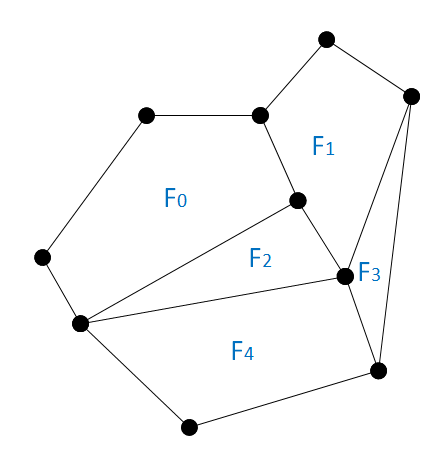
\includegraphics[width=6cm]{images/ch2/PolygonMeshExample}
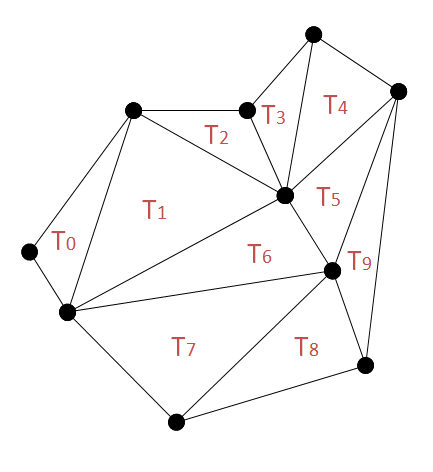
\includegraphics[width=6cm]{images/ch2/TriangleMeshExample}
\caption{Left: Polygonal Mesh, Right: Triangulated Mesh}
\label{MeshExamples}
\end{figure}


The Feature-Oriented Geometric Progressive Lossless Mesh coder (FOLProM) \cite{Peng10Feature} is a state of the art codec which is progressive. It also aims to be an effective low-bitrate codec. It classifies segments of the mesh as being visually salient or not. Salient segments are preserved more during compression compared to non-salient ones. \\

Karni and Gotsman \cite{Karni00Spectral} proposed a lossy method which compresses a spectral representation of a mesh. This algorithm generally partitions the mesh and compresses each partition separately since it does not work on large meshes. Encoding a basis function for each partition, coefficients are quantized, truncated and entropy coded. Results show this method outperforms the previous state of the art valence method \cite{touma98triangle} at coarse quantization levels. Bayazit et al. \cite{Bayazit103DMesh} also developed a progressive method based on spectral compression. This method is based on the region adaptive transform in the spectral domain and is advertised as a current state of the art lossy 3D data compression method. \\

A lossy wavelet based compression system was proposed by Khodakovsky et al \cite{Khodakovsky00Progressive}. This technique samples the mesh, and uses the wavelet transform to decorrelate the data. Coefficients are quantized and stored in a structure called a zero tree which increases compression performance. This method is also shown to outperform the valence method. Other wavelet approaches \cite{Guskov00Normal,Khodakovsky04Normalmesh} also sample the mesh and use a multi-resolution representation in which the data is described using local normal directions on the mesh surface. \\


\subsubsection{Point Cloud}

The point cloud structure stores a list of 3D points. This representation can be thought of as discrete samples of the surface of a real 3D object. Figure \ref{PointCloudExample} shows an example. This structure can be sampled using a variety of methods. These methods include both dense and sparse sampling, and sample steps can be either regular or irregular. Along with each vertex, a variety of attribute information can be stored. Point cloud data may be obtained via a 3D scanner or RGB-D camera. 

\begin{figure}[!h]
\centering
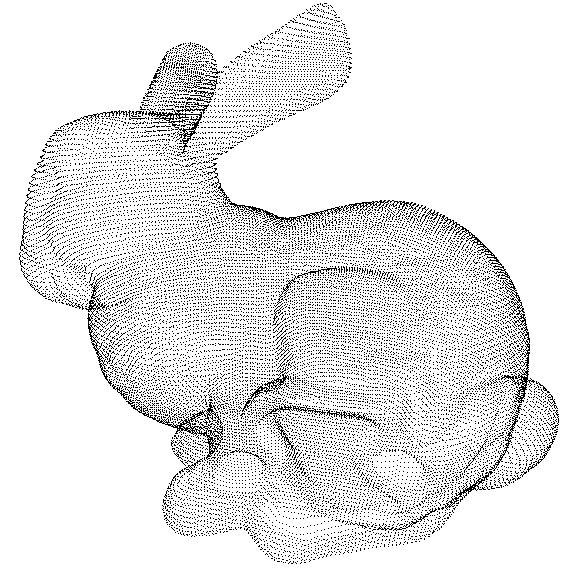
\includegraphics[width=6cm]{images/ch2/PointCloudExample}
\caption{A densely sampled point cloud of the Stanford Bunny.}
\label{PointCloudExample}
\end{figure}


\subsubsection{3D Volume}

In this representation, points are sampled into a 3D cubic space of sub-cubes called voxels. Such a space may have separate dimensions for width, height and depth or the space may be a true cube. In the context of 3D reconstruction, this data-representation is common and is used to store boolean values describing the occupancy of a space \cite{Rusinkiewicz02Real}. A visualization of a 3D volume showing a reconstruction is shown in figure [WARNING: Insert Graphic here]. This data type is useful because it allows for quick updates. Downsides include, large storage space and the fact that 3D space represented cannot be dynamically changed without significant cost. \\


\subsubsection{Signed Distance Functions}

A Signed Distance Function \cite{Curless96Volumetric} is a function which describes a 3D geometric space. Such a function takes a 3D location as $x,y,z$ coordinates as input and returns a single number value. The value describes the geometric detail of a particular object. Zero values are surface interfaces, positive values increase relative to the distance to the nearest surface and negative values represent the interior of the object. \\

SDFs may take the form of an equation or may be made discrete by means of discretization. In the context of 3D reconstruction we refer to the discrete SDF, an example of which is show in figure [WARNING : insert a figure]. The SDF may be visualized by converting it to a mesh and rendering (by means of the marching cubes algorithm \cite{Cubes87High}) or by directly ray-casting the structure \cite{Parker98Interactive}. In the case of ray-casting, there is a significant advantage over the volumetric representation, that is the step size may be adjusted dynamically reducing render time. \\

Canelhas \cite{Canelhas12Scene} did a masters thesis on an approach for camera tracking which makes use of an SDF. Similar to the work by Bylow et al \cite{Bylow13Real} the project concentrates on object detection and recognition in an SDF although little evaluation was performed. Additionally storage was not considered. Kubacki \cite{Kubacki12Registration} proved the SDF is useful in estimating camera pose but only showed proof using synthetic data performing no comparative evaluation. Ren and Reid \cite{Ren12Unified}  demonstrated SDF based object tracking based on prior known models. \\

Elfes et al \cite{Elfes87Sensor} use a Baysian probability of occupancy measure to decide if a point should be added to the grid and showed that SDFs may be used to fuse partial depth scans whilst impeding problems with mesh based reconstruction algorithms. The SDF representation was modified by Zach et al \cite{Zach07Globally} to be more robust to noise. Bylow et al noted that the SDF may be used to produce globally satisfied reconstructions in real time. \\


\subsubsection{Image Based Representations}

3D reconstructions may also be represented by means of elevation maps \cite{Herbert89Terrain} and multi-level surface maps \cite{Triebel06Multi} however these methods cannot store known and unknown areas of occupancy in a volumetric way. Additionally compression is often not considered and these methods do not have the search capabilities which the Octree and volumetric representations have, nor the fine detail available in a mesh or point cloud representation. An example of an elevation map is shown in figure [WARNING: insert figure here]\\

Gu et al \cite{Gu02Geometry} devised a solution for representing 3D models as 2D images which are then compressed using state of the art image compression methods (based on wavelets). To form this representation, the mesh is cut along a network of edge paths, opening the mesh into a topological disk, which is then sampled onto a 2D grid. Each pixel in the image has a corresponding coordinate in the model, with pixel neighbourhoods describing connectivity. Comparisons with the method by Khodakovsky et al reveal the geometry image codec does not have as high compression performance. \\


\subsubsection{Octree}

The Octree is a hierarchical data representation ideal for storage, search and processing of 3D data. Other hierarchical structures exist (such as K-D tree and BSP-tree) \cite{Samet06Foundations} but these are not as useful for compression as the Octree, which is the aim of this research. The Octree is described in detail below in section \ref{OTDesc}. An important technique based on the Octree and used by many 3D reconstruction methods is the Octomap \cite{Wurm10Octomap}. It essentially records a volume occupancy grid using an Octree. This method models data probabilistically whilst simultaneously reducing memory size. The Octomap representation is lossless and is can reduce the file size of the reconstruction by up to 50\%. \\

Other methods also explore the Octree for 3D reconstruction and SLAM \cite{9,Fournier07Mapping,Meagher82Geometric,Fairfield07Real} however these methods do not really address storage advantages. 



